\documentclass[11pt]{article}
\usepackage[textwidth=18.0cm, textheight=23.0cm, top=2.0cm]{geometry}
\usepackage{pst-all}
\usepackage{amssymb}
\usepackage{tikz}
\usepackage{underscore}\begin{document}
\pagestyle{empty}


ClassName: \underline{\textbf{Class_07.2bp-3}}
\par
BinSize: \underline{\textbf{100 × 100}}
\par
ReduceSize: \underline{\textbf{100 × 99}}
\par
TypeNum: \underline{\textbf{19}}
\par
Num: \underline{\textbf{20}}
\par
OutS: \underline{\textbf{70000}}
\par
InS: \underline{\textbf{51044}}
\par
Rate: \underline{\textbf{0.729}}
\par
UB: \underline{\textbf{7}}
\par
LB0: \underline{\textbf{7}}
\par
LB: \underline{\textbf{7}}
\par
LBWithCut: \underline{\textbf{7}}
\par
NodeCut: \underline{\textbf{0}}
\par
ExtendedNodeCnt: \underline{\textbf{1}}
\par
GenNodeCnt: \underline{\textbf{1}}
\par
PrimalNode: \underline{\textbf{0}}
\par
ColumnCount: \underline{\textbf{7}}
\par
TotalCutCount: \underline{\textbf{0}}
\par
RootCutCount: \underline{\textbf{0}}
\par
LPSolverCnt: \underline{\textbf{1}}
\par
PricingSolverCnt: \underline{\textbf{0}}
\par
BranchAndBoundNum: \underline{\textbf{1}}
\par
isOpt: \underline{\textbf{true}}
\par
TimeOnPrimal: \underline{\textbf{0.000 s}}
\par
TimeOnPricing: \underline{\textbf{0.000 s}}
\par
TimeOnRmp: \underline{\textbf{0.062 s}}
\par
TotalTime: \underline{\textbf{0.125 s}}
\par
\newpage


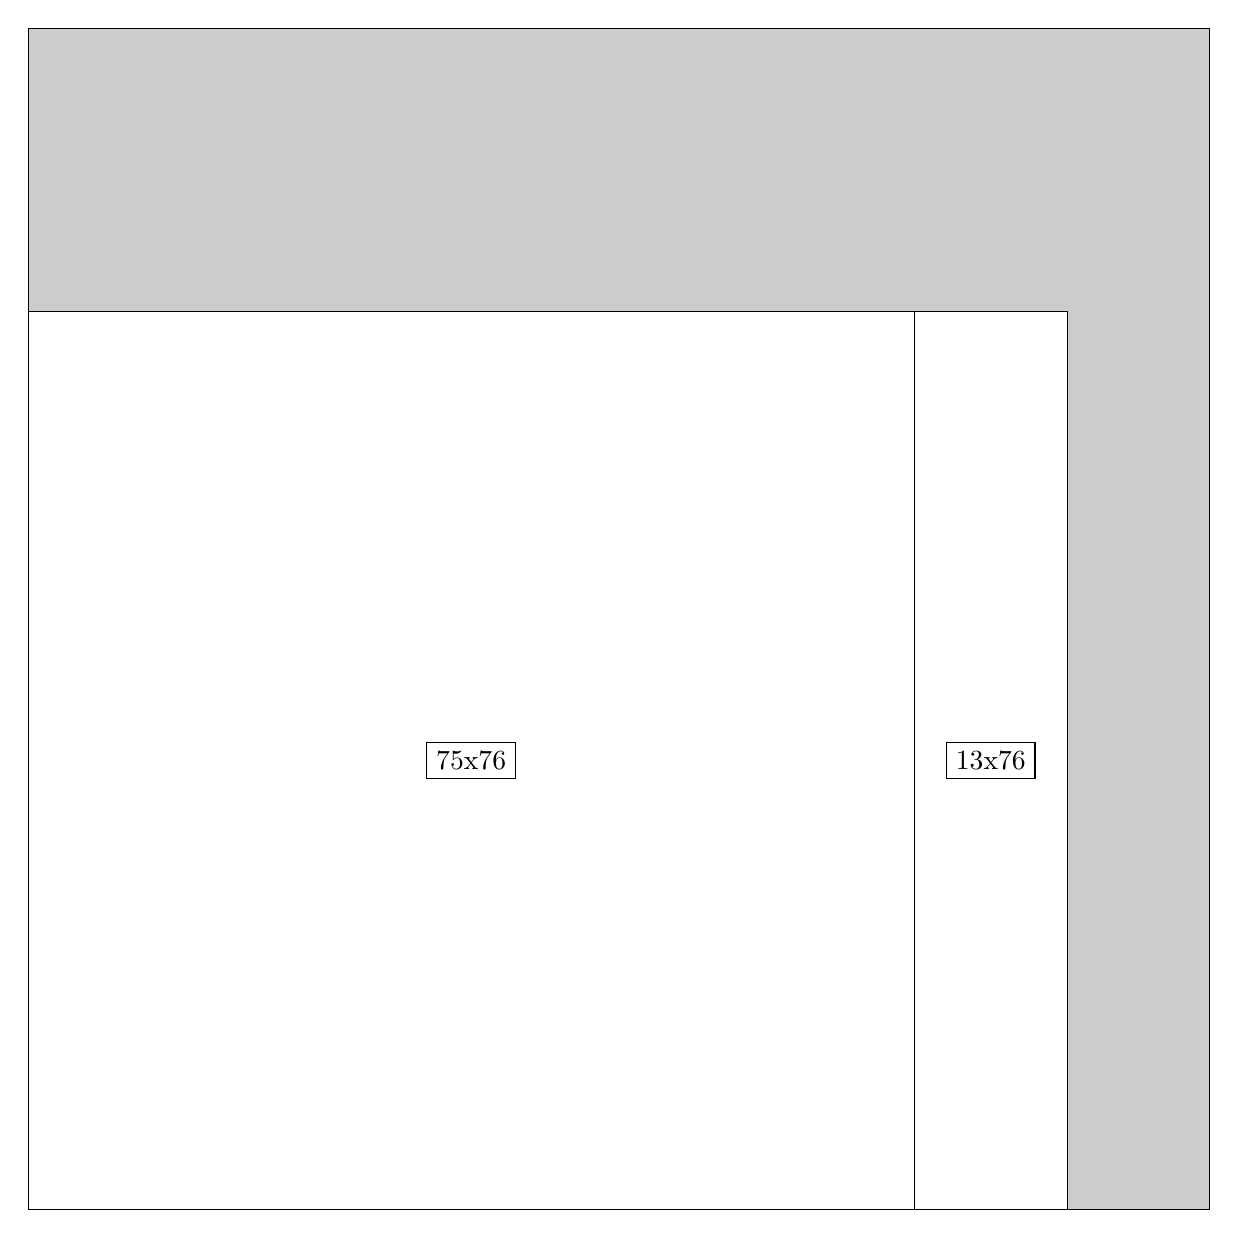
\begin{tikzpicture}[shorten >=1pt,scale=1.0,every node/.style={scale=1.0},->]
\tikzstyle{vertex}=[circle,fill=black!25,minimum size=14pt,inner sep=0pt]
\filldraw[fill=gray!40!white, draw=black] (0,0) rectangle (15.0,15.0);
\foreach \name/\x/\y/\w/\h in {75x76/0.0/0.0/11.25/11.4,13x76/11.25/0.0/1.95/11.4}
\filldraw[fill=white!40!white, draw=black] (\x,\y) rectangle node[draw] (\name) {\name} ++(\w,\h);
\end{tikzpicture}


w =75 , h =76 , x =0 , y =0 , v =5700
\par
w =13 , h =76 , x =75 , y =0 , v =988
\par
\newpage


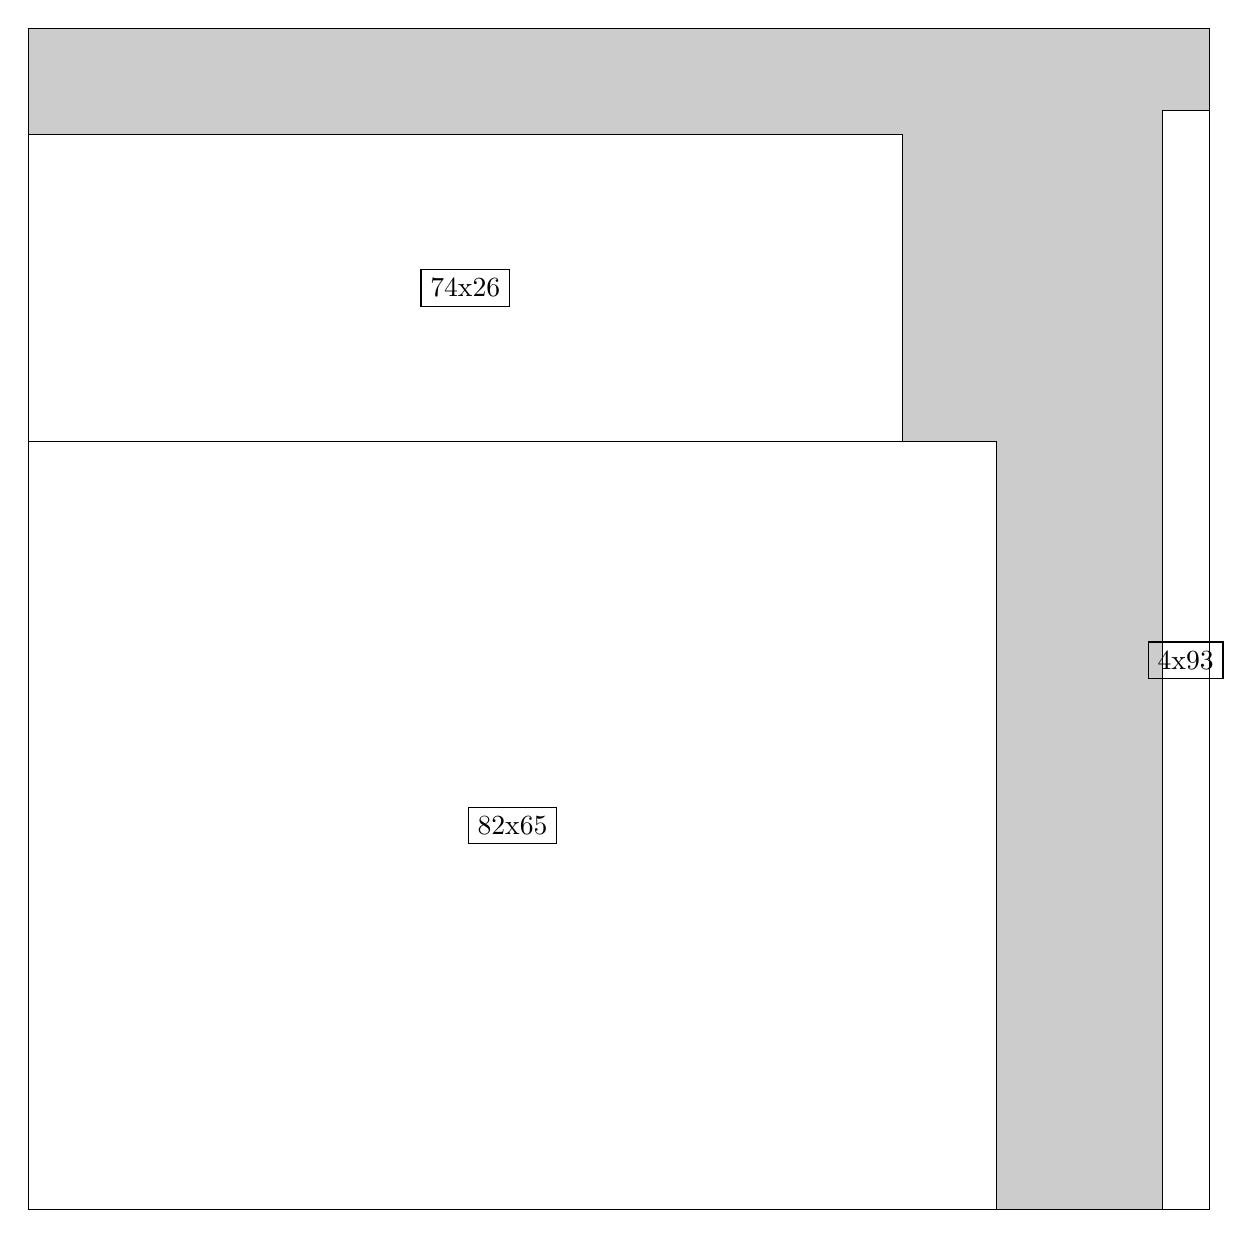
\begin{tikzpicture}[shorten >=1pt,scale=1.0,every node/.style={scale=1.0},->]
\tikzstyle{vertex}=[circle,fill=black!25,minimum size=14pt,inner sep=0pt]
\filldraw[fill=gray!40!white, draw=black] (0,0) rectangle (15.0,15.0);
\foreach \name/\x/\y/\w/\h in {82x65/0.0/0.0/12.299999999999999/9.75,74x26/0.0/9.75/11.1/3.9,4x93/14.399999999999999/0.0/0.6/13.95}
\filldraw[fill=white!40!white, draw=black] (\x,\y) rectangle node[draw] (\name) {\name} ++(\w,\h);
\end{tikzpicture}


w =82 , h =65 , x =0 , y =0 , v =5330
\par
w =74 , h =26 , x =0 , y =65 , v =1924
\par
w =4 , h =93 , x =96 , y =0 , v =372
\par
\newpage


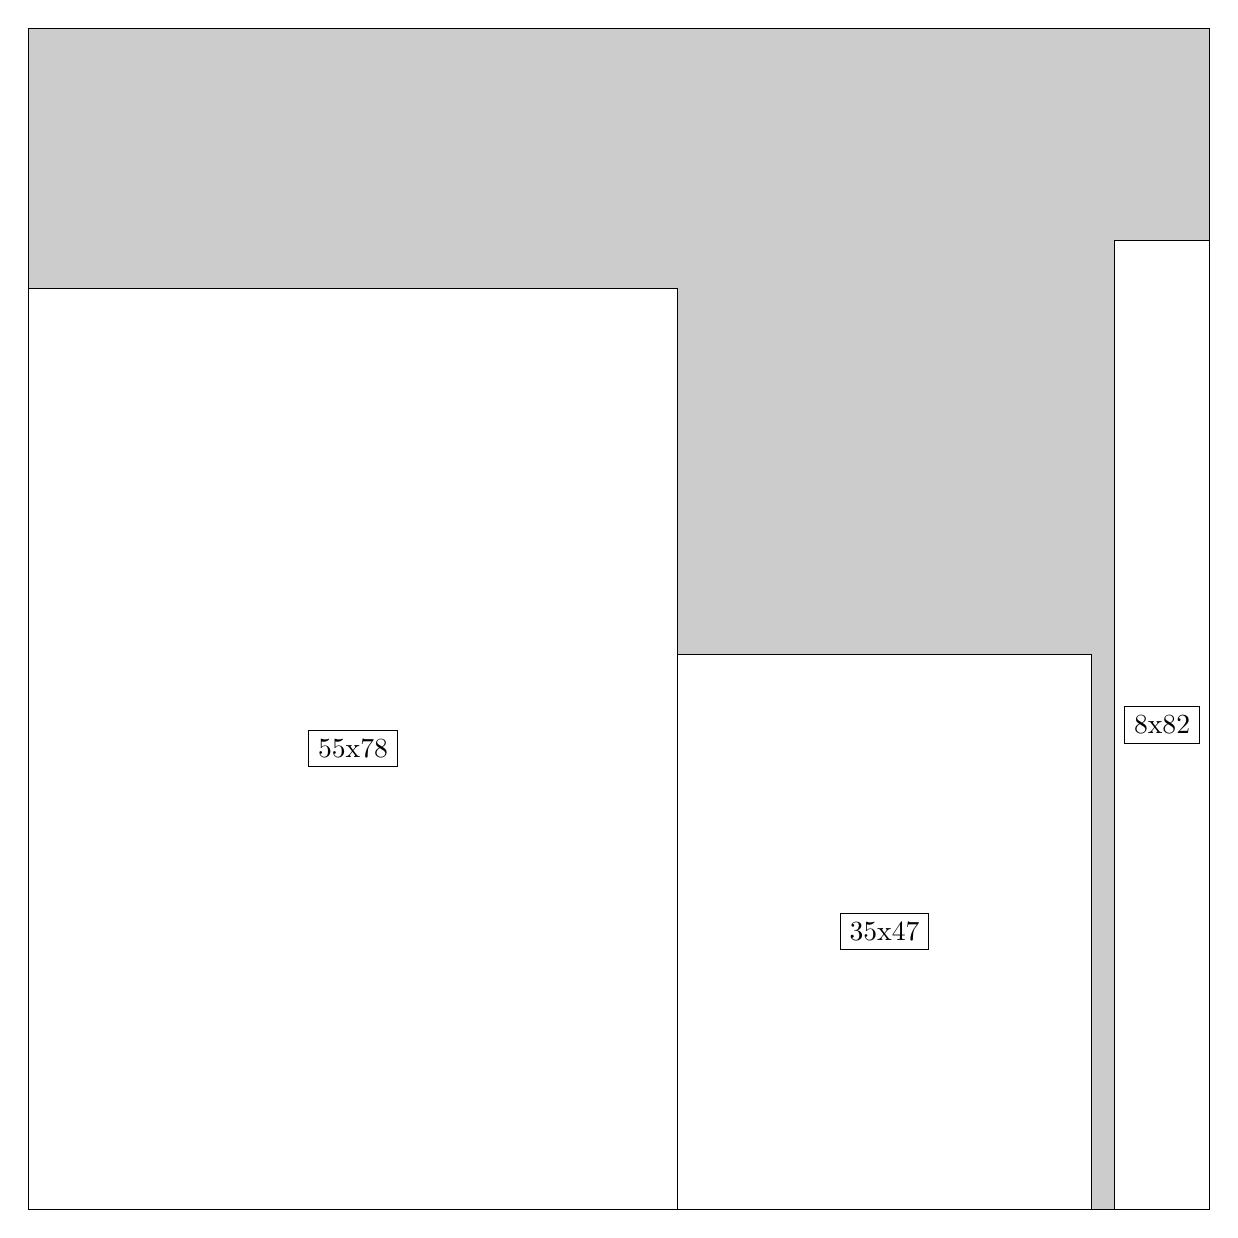
\begin{tikzpicture}[shorten >=1pt,scale=1.0,every node/.style={scale=1.0},->]
\tikzstyle{vertex}=[circle,fill=black!25,minimum size=14pt,inner sep=0pt]
\filldraw[fill=gray!40!white, draw=black] (0,0) rectangle (15.0,15.0);
\foreach \name/\x/\y/\w/\h in {35x47/8.25/0.0/5.25/7.05,55x78/0.0/0.0/8.25/11.7,8x82/13.799999999999999/0.0/1.2/12.299999999999999}
\filldraw[fill=white!40!white, draw=black] (\x,\y) rectangle node[draw] (\name) {\name} ++(\w,\h);
\end{tikzpicture}


w =35 , h =47 , x =55 , y =0 , v =1645
\par
w =55 , h =78 , x =0 , y =0 , v =4290
\par
w =8 , h =82 , x =92 , y =0 , v =656
\par
\newpage


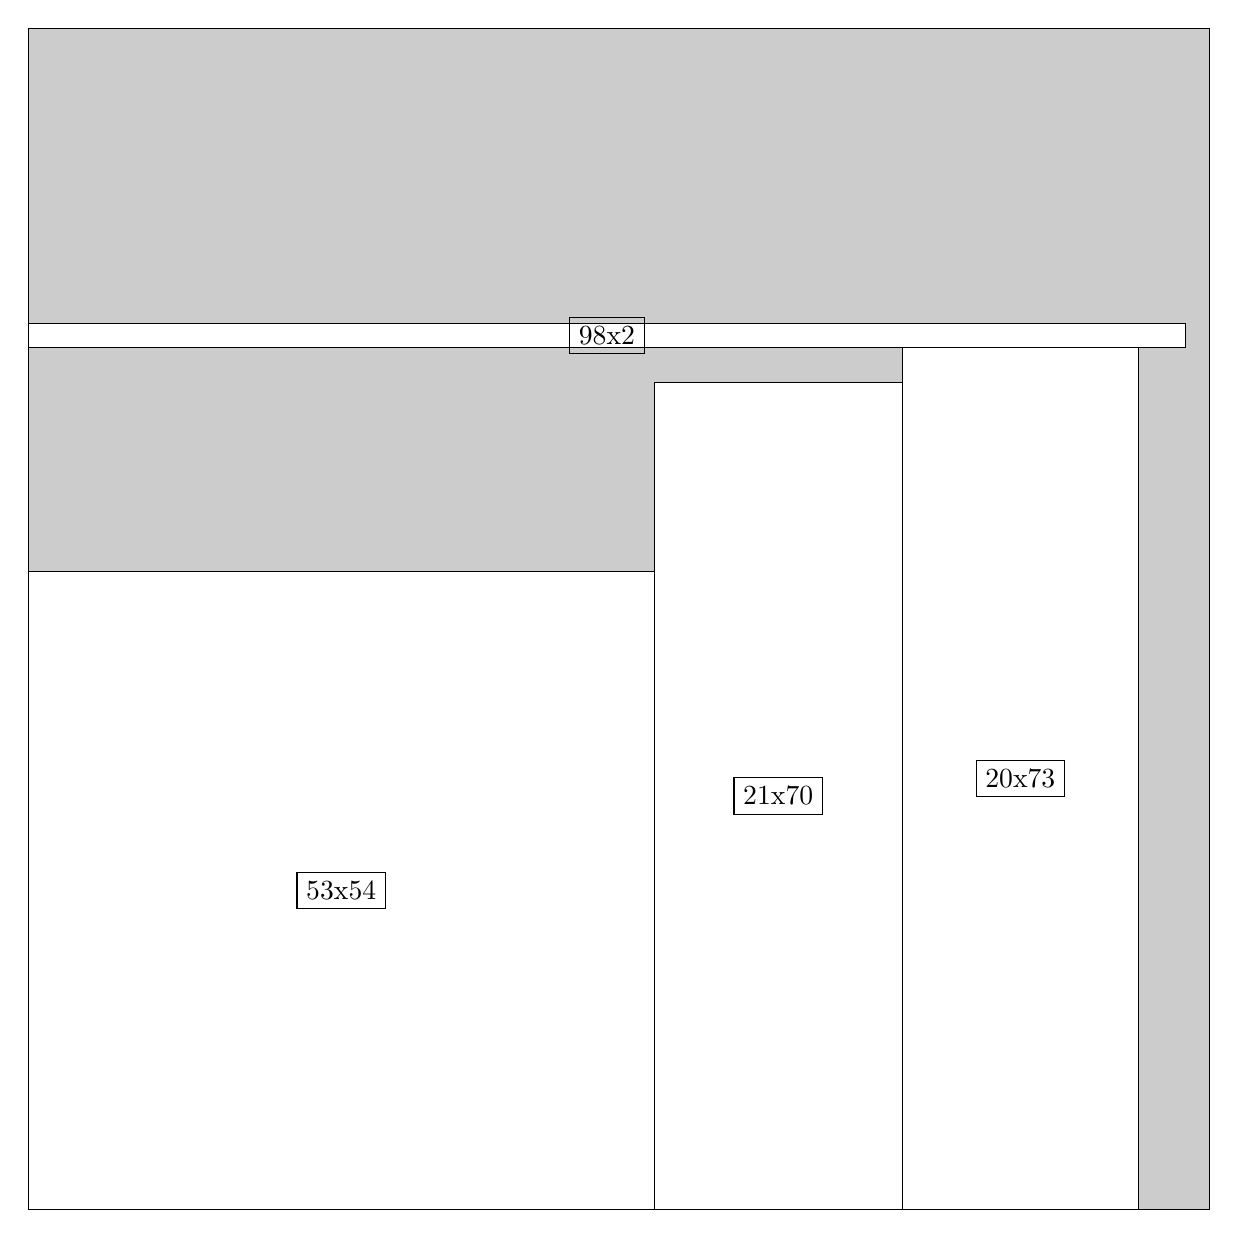
\begin{tikzpicture}[shorten >=1pt,scale=1.0,every node/.style={scale=1.0},->]
\tikzstyle{vertex}=[circle,fill=black!25,minimum size=14pt,inner sep=0pt]
\filldraw[fill=gray!40!white, draw=black] (0,0) rectangle (15.0,15.0);
\foreach \name/\x/\y/\w/\h in {53x54/0.0/0.0/7.949999999999999/8.1,21x70/7.949999999999999/0.0/3.15/10.5,20x73/11.1/0.0/3.0/10.95,98x2/0.0/10.95/14.7/0.3}
\filldraw[fill=white!40!white, draw=black] (\x,\y) rectangle node[draw] (\name) {\name} ++(\w,\h);
\end{tikzpicture}


w =53 , h =54 , x =0 , y =0 , v =2862
\par
w =21 , h =70 , x =53 , y =0 , v =1470
\par
w =20 , h =73 , x =74 , y =0 , v =1460
\par
w =98 , h =2 , x =0 , y =73 , v =196
\par
\newpage


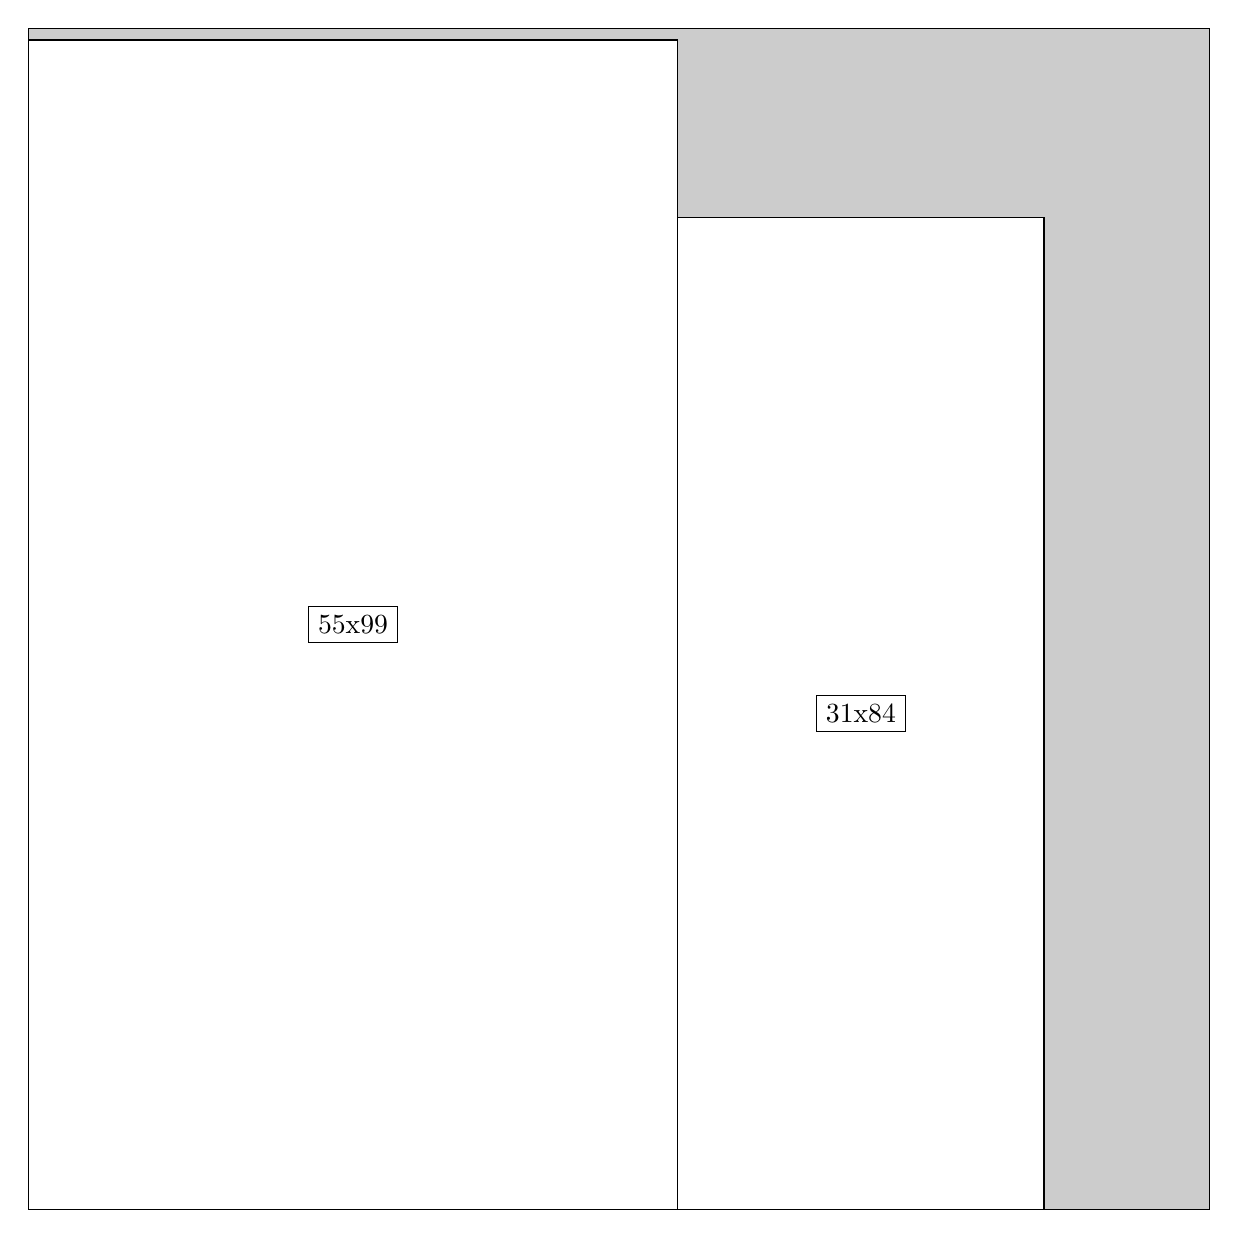
\begin{tikzpicture}[shorten >=1pt,scale=1.0,every node/.style={scale=1.0},->]
\tikzstyle{vertex}=[circle,fill=black!25,minimum size=14pt,inner sep=0pt]
\filldraw[fill=gray!40!white, draw=black] (0,0) rectangle (15.0,15.0);
\foreach \name/\x/\y/\w/\h in {31x84/8.25/0.0/4.6499999999999995/12.6,55x99/0.0/0.0/8.25/14.85}
\filldraw[fill=white!40!white, draw=black] (\x,\y) rectangle node[draw] (\name) {\name} ++(\w,\h);
\end{tikzpicture}


w =31 , h =84 , x =55 , y =0 , v =2604
\par
w =55 , h =99 , x =0 , y =0 , v =5445
\par
\newpage


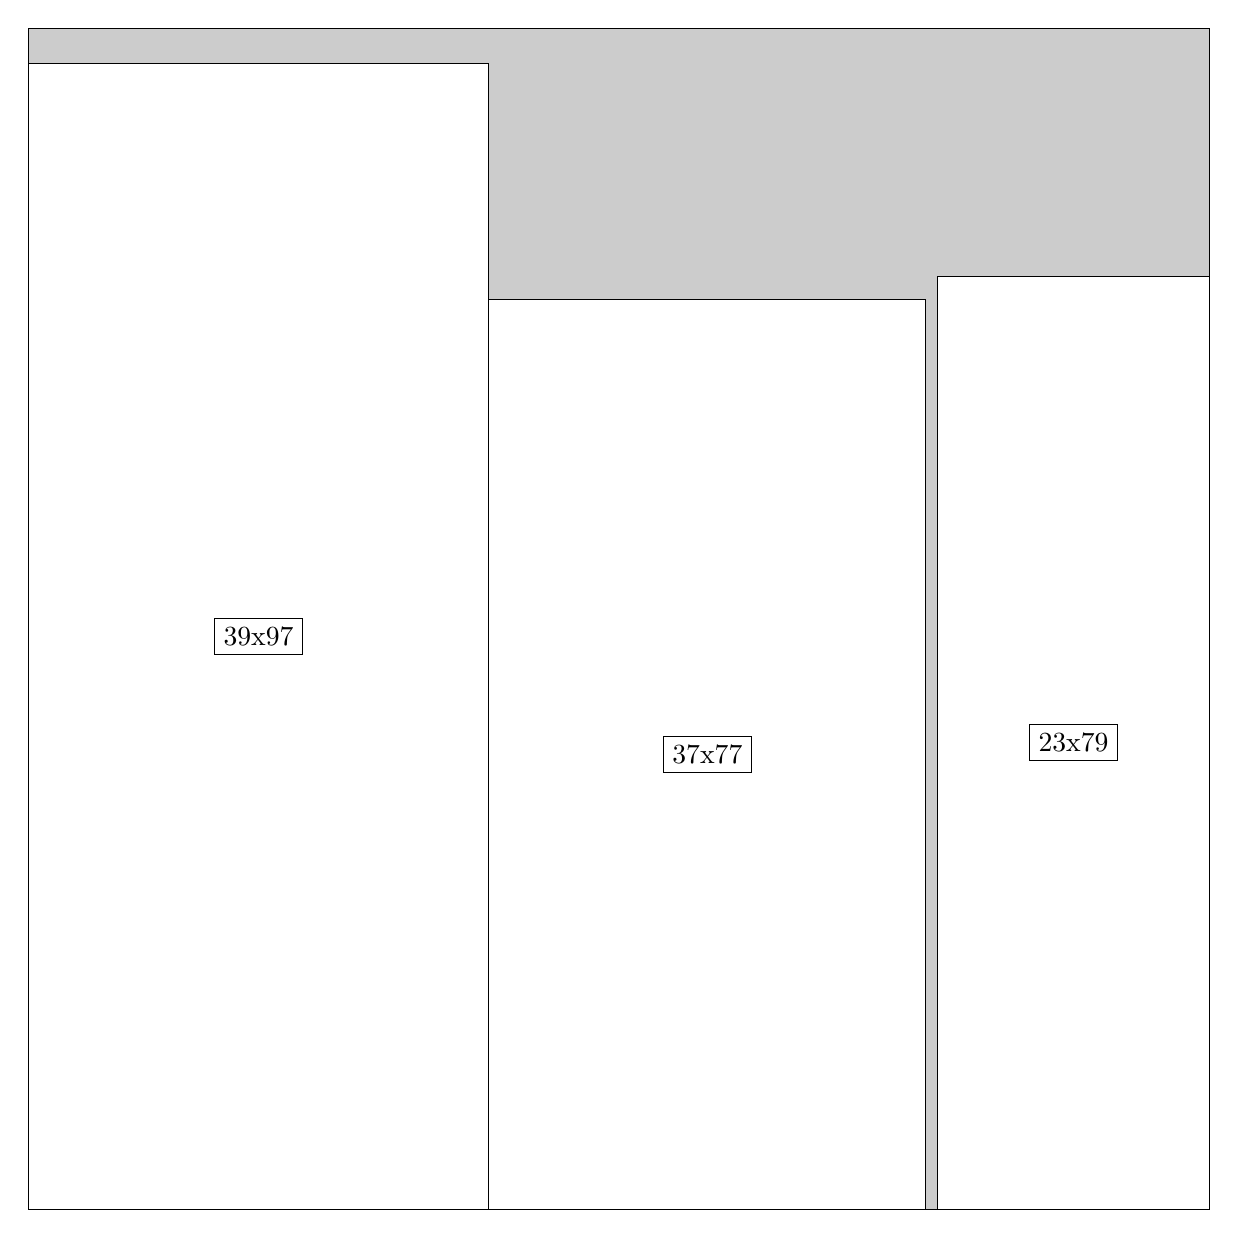
\begin{tikzpicture}[shorten >=1pt,scale=1.0,every node/.style={scale=1.0},->]
\tikzstyle{vertex}=[circle,fill=black!25,minimum size=14pt,inner sep=0pt]
\filldraw[fill=gray!40!white, draw=black] (0,0) rectangle (15.0,15.0);
\foreach \name/\x/\y/\w/\h in {39x97/0.0/0.0/5.85/14.549999999999999,37x77/5.85/0.0/5.55/11.549999999999999,23x79/11.549999999999999/0.0/3.4499999999999997/11.85}
\filldraw[fill=white!40!white, draw=black] (\x,\y) rectangle node[draw] (\name) {\name} ++(\w,\h);
\end{tikzpicture}


w =39 , h =97 , x =0 , y =0 , v =3783
\par
w =37 , h =77 , x =39 , y =0 , v =2849
\par
w =23 , h =79 , x =77 , y =0 , v =1817
\par
\newpage


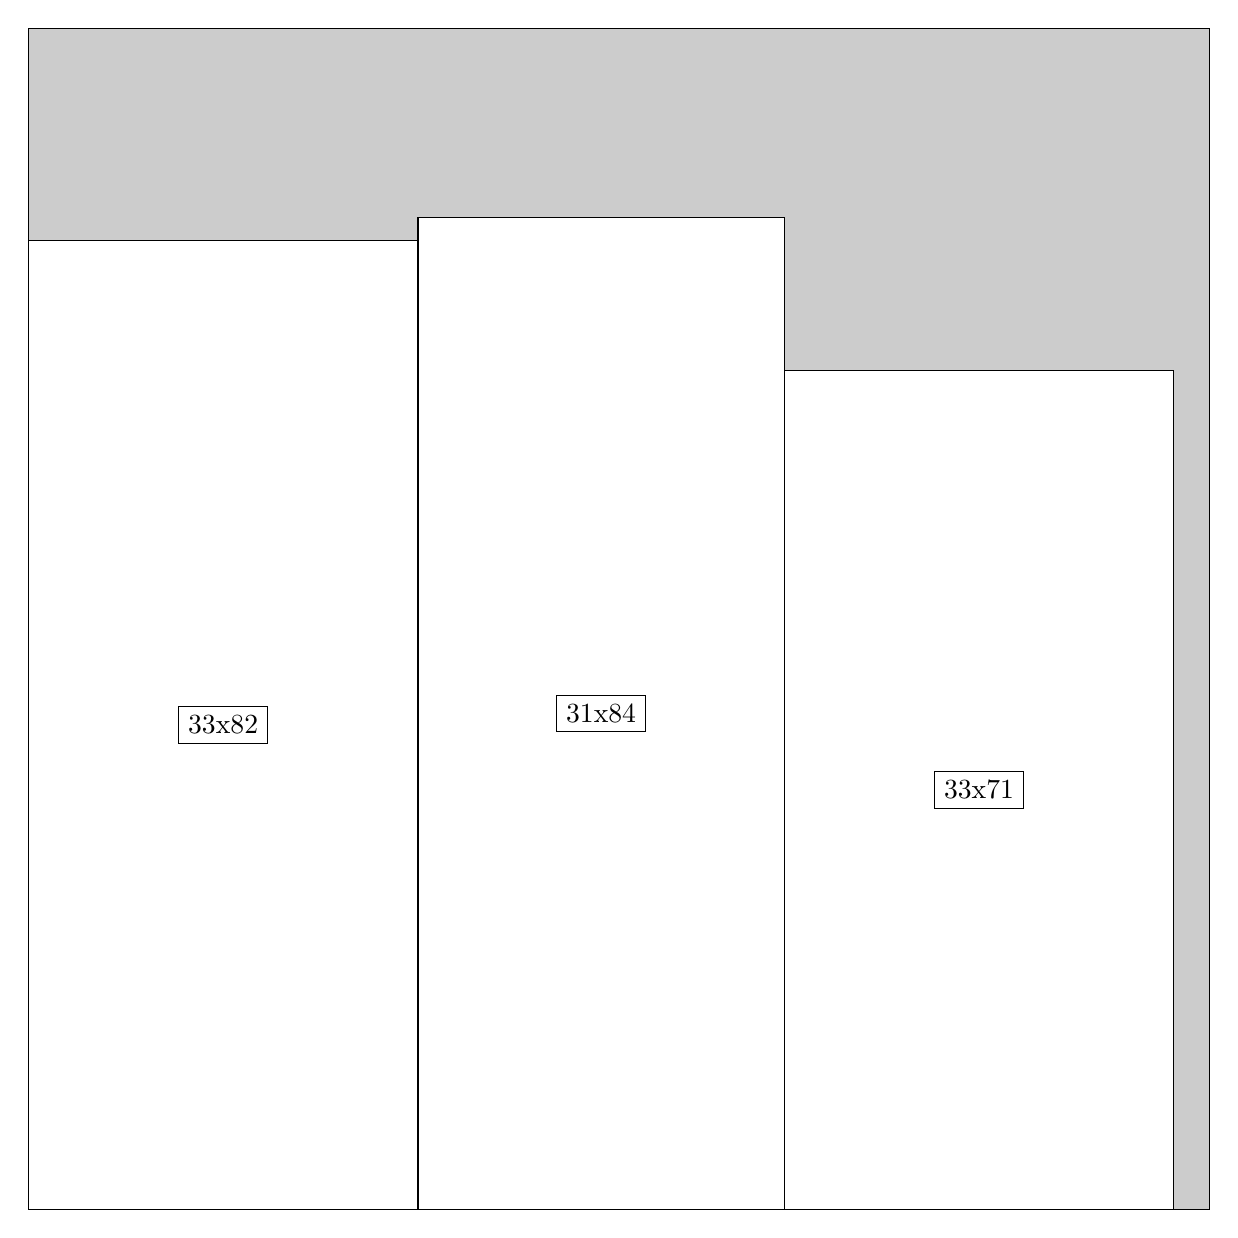
\begin{tikzpicture}[shorten >=1pt,scale=1.0,every node/.style={scale=1.0},->]
\tikzstyle{vertex}=[circle,fill=black!25,minimum size=14pt,inner sep=0pt]
\filldraw[fill=gray!40!white, draw=black] (0,0) rectangle (15.0,15.0);
\foreach \name/\x/\y/\w/\h in {33x82/0.0/0.0/4.95/12.299999999999999,31x84/4.95/0.0/4.6499999999999995/12.6,33x71/9.6/0.0/4.95/10.65}
\filldraw[fill=white!40!white, draw=black] (\x,\y) rectangle node[draw] (\name) {\name} ++(\w,\h);
\end{tikzpicture}


w =33 , h =82 , x =0 , y =0 , v =2706
\par
w =31 , h =84 , x =33 , y =0 , v =2604
\par
w =33 , h =71 , x =64 , y =0 , v =2343
\par
\newpage


\end{document}